%NOTE: main file of the latex eg. entries 
\documentclass[12pt,a4paper]{article}

%\setlength{\headheight}{210pt} 

\usepackage[letterpaper]{geometry}
\usepackage{times}
\geometry{top=1.0in, bottom=1.5in, left=1.0in, right=1.0in}

\usepackage{fancyhdr}
\pagestyle{fancy}
\lhead{} 

\rhead{
\begin{tabular}{c}
\textsc
Group 3 \\
Trinity \\
VG100
\end{tabular}
}

\chead{} 
\lfoot{} 
\cfoot{} 
\rfoot{} 
\renewcommand{\headrulewidth}{0pt} 
\renewcommand{\footrulewidth}{0pt} 

\setlength\headsep{0.333in}

\usepackage{fontspec}
\setmainfont{Times New Roman}

\usepackage{graphicx}

\usepackage{hyperref}

\usepackage{caption}

\usepackage{indentfirst}

\usepackage{setspace}

\title{Group3P1Manual}
\author{Ren Wang}

% ===========================================

\begin{document}


% ===========================================


%NOTE: cover page
\begin{center}
\vspace*{0.7in}
%\includegraphics[width=0.55\textwidth]{./pot}\\[1cm]    
\vspace*{0.7in}

%\textsc{\Large Major Research Paper}\\[0.5cm]


% Title


% Author and supervisor

\begin{center} 


\includegraphics[height=3cm]{picture/umjiLogo}


{
\linespread{2}
\LARGE
\textsc{VG100 Introduction To Engineering} \\
}
{
\Large
\textsc{Project 1 Bridge Crane} \\
}


\vspace*{0.6in}

\textsc{\large Group 3 Trinity}\\

\vspace*{0.2in}


\begin{tabular}{cc}
{\fontspec{Hei}\selectfont 谢舒翔} & Shuxiang \textsc{Xie} \\
{\fontspec{Hei}\selectfont 郭成彰} & Chengzhang \textsc{Guo} \\
{\fontspec{Hei}\selectfont 麻珂睿} & Kerui \textsc{Ma} \\
{\fontspec{Hei}\selectfont 王韧} & Ren \textsc{Wang} \\
{\fontspec{Hei}\selectfont 朱波颖} & Boying \textsc{Zhu} \\
\end{tabular}


\vspace*{0.5in}

\begin{tabular}{cc}
Professor & Yanfeng \textsc{Shen} \\
Professor & Cynthia \textsc{Vagnetti} 
\end{tabular}


\vspace*{0.7in}

{\today}


\end{center}



% Bottom of the page
\end{center}
\newpage
% NOTE: end of cover page


% =============================

\lhead{%
  
\includegraphics[height=1cm]{picture/umjiLogo}
}

\rhead{
  \raisebox{2ex}{%
    \begin{tabular}{cl}
    Prof. & Yanfeng \textsc{Shen} \\
    Prof. & Cynthia \textsc{Vagnetti} 
    \end{tabular}
  }
}

\cfoot{
  
\includegraphics[height=1cm]{picture/teamLogo}  
  \raisebox{2ex}{Group 3}%
}
\rfoot{
  \thepage
}

\renewcommand{\headrulewidth}{0.4pt} 
\renewcommand{\footrulewidth}{0pt} 

% =============================

\onehalfspacing
\tableofcontents
\newpage

% =============================

\doublespacing
\section{Introduction}

\subsection{About Us and Campus}


\begin{figure}[htbp]
\centering
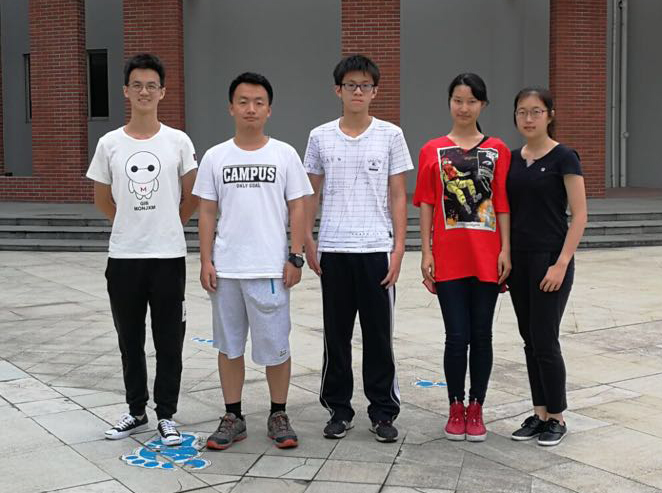
\includegraphics[height=8cm]{picture/teamMember}
  \caption{Our team \label{fig:teamMember}}
\end{figure}

We are TRINITY (Figure \ref{fig:teamMember}), a team of freshmen from University of
Michigan-Shanghai Jiao Tong University Joint Institute (UM-SJTU JI), which is
located in the campus of Shanghai Jiao Tong University (Figure
\ref{fig:campus}). People in the photo are Xie Shuxiang, Zhu Boying, Ma Kerui,
Wang Ren and Guo Chengzhang, and our group leader is Xie Shuxiang. Joint
Institute is well-known for its unique way of helping students develop the
ability of cooperation and innovation. As a result, students here have various
projects and activities to attend to broaden their horizons.  


\begin{figure}[htbp]
\centering
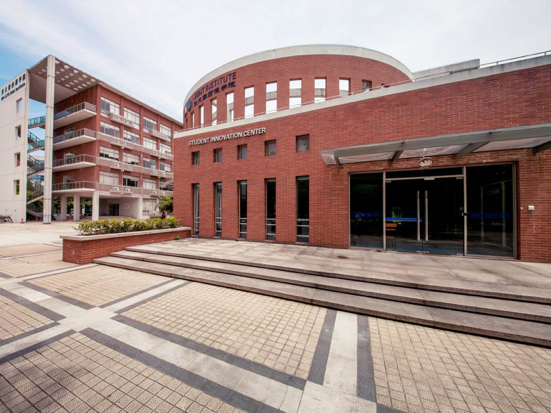
\includegraphics[height=5cm]{figure/campus}
  \caption{\label{fig:campus}}
\end{figure}

\subsection{Course and Project Information}


VG100 is a course about Introduction to Engineering. It is a mandatory course
for all freshmen in JI. According to Professor Shen Yanfeng, the course not only
convey fundamental knowledge of engineering, but also help students learn how to
solve a realistic problem. Besides, the technical communication part strengthens
students’ ability of taking part in teamwork, which is of great importance for
engineers.  

The first project students should accomplish in VG100 is to make a bridge-crane
system. It should be able to allow a cart to pull a cup of water up, travel
forward on the bridge to the other side, and put down the cup of water on the
designated place (Figure \ref{fig:structureOfP1}).  

\begin{figure}[htbp]
\centering
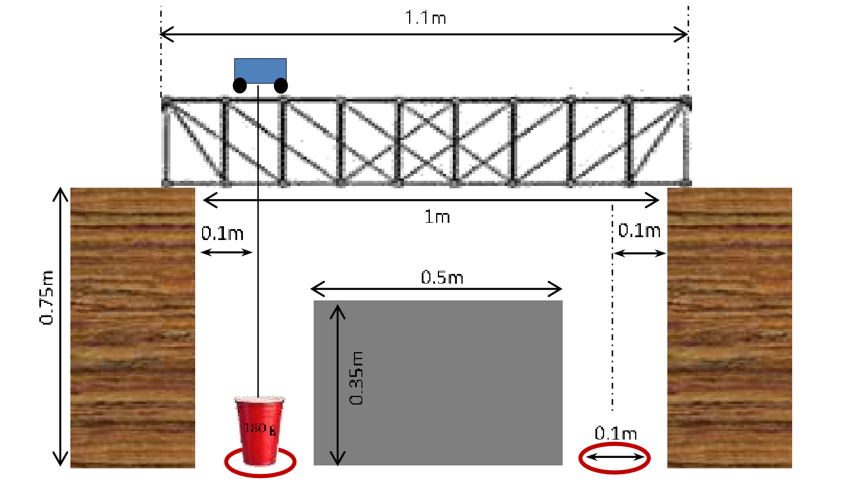
\includegraphics[height=5cm]{figure/structureOfP1}
\caption{\label{fig:structureOfP1}}
\end{figure}

The following list from the professor shows the specific requirement of Project 1.
Mechanism: Any method that can achieve the above task will be acceptable.
Breaking any of these rules will result in failing project 1.  
Bridge length:  >= 1.1m 
Bridge width:  <= 0.2 m 
Bridge Material: printing paper (80g size A4) and non-toxic, white wood glue
(brand: LongMa). Any additional material violates the rule!  
Maximum Mass of the bridge: 200g 
Maximum length of the cart: 0.1 m 
Power Supply: Maximum two portable Power Supply (for each battery Voltage ≤ 12V) 
Motor specifications: < 12V.  
Central Control Circuit: Arduino series (Required for Programming \& Can Be Omitted)

\subsection{Race Performance}
(This part will be completed later)

 % introduction
\newpage
\input{part/designOverview} % design overview
\newpage
\section{Materials \& Tools}
% images
\newcommand{\beginMyTabular}{
    \begin{center}
    \begin{tabular}{p{0.4cm}p{5cm}p{5cm}rr}
    \hline
    No. & Item & Specification & Quantity & Price(Yuan) \\
    \hline
}
\newcommand{\MyTabularEnd}{
    \hline
    \end{tabular}
    \end{center}
}
% counter
\newcounter{matcnt}
\setcounter{matcnt}{0}
\newcommand{\CounterOfM}{
    \stepcounter{matcnt}\arabic{matcnt}
}
% CounterOfM means the counter of materials
%
\newcounter{figcnt}
\setcounter{figcnt}{0}
\newcommand{\CounterOfF}{
    \stepcounter{figcnt}\arabic{figcnt}
}
\newcommand{\CounterOfFa}[1]{
    \raisebox{#1cm}{
        \fbox{\small \CounterOfF} \hspace{0.3cm}
    }
    \nolinebreak[3]
}
\newcommand{\MPGx}[3]{
    \CounterOfFa{#1}
	\begin{minipage}{0.2\textwidth}
    \centering    
    \includegraphics[height=#2cm]{picture/material/#3}
    \end{minipage}
}
\newcommand{\MPGxA}[3]{
    \CounterOfFa{#1}
	\begin{minipage}{0.1\textwidth}
    \centering    
    \includegraphics[height=#2cm]{picture/material/#3}
    \end{minipage}
}
%% ====================================================
%% ====================================================
%% ====================================================
\newcommand{\HPRx}{1.4}
\newcommand{\HPx}{2}
\newcommand{\MyWidthFirstLine}{3.3cm}

%\begin{flushleft}
%\begin{tabular}{p{\MyWidthFirstLine}p{\MyWidthFirstLine}p{\MyWidthFirstLine}p{\MyWidthFirstLine}}
%\end{tabular}
%\end{flushleft}
%
\begin{center}
\begin{tabular}{lll}
\MPGxA{\HPRx}{\HPx}{a4paper} & \MPGxA{\HPRx}{\HPx}{whiteglue} & \MPGxA{\HPRx}{\HPx}{papercutter} \\
\MPGxA{\HPRx}{\HPx}{brush} & \MPGx{\HPRx}{\HPx}{woodstick} & \MPGx{\HPRx}{\HPx}{scissor} \\
\MPGx{\HPRx}{\HPx}{arduino} & \MPGx{\HPRx}{\HPx}{standN20} & \MPGx{\HPRx}{\HPx}{moterN20} \\
\MPGx{\HPRx}{\HPx}{wheelrubber} & \MPGx{\HPRx}{\HPx}{servo360} & \MPGx{\HPRx}{\HPx}{batteryPlane} \\
\MPGx{\HPRx}{\HPx}{batteryBreeze} & \MPGx{\HPRx}{\HPx}{switch} & \MPGx{\HPRx}{\HPx}{pcbBoard} \\  
\MPGx{\HPRx}{\HPx}{tapeThick} & \MPGx{\HPRx}{\HPx}{stringYoYo} & \MPGx{\HPRx}{\HPx}{m3} \\ 
\MPGx{\HPRx}{\HPx}{m2} & \MPGx{\HPRx}{\HPx}{car} \\
\end{tabular}
%
\end{center}
%
\subsection{Bridge}
\subsubsection{Materials}
% tables
\beginMyTabular
\CounterOfM & A4 paper & Double A 80 g  A4 paper  & 10 & 29.8 \\
\CounterOfM & Long Ma White Glue & 400 g & 5 & 67.5 \\
\MyTabularEnd

\subsubsection{Tools}

% images

% tables
\beginMyTabular
\CounterOfM & Huanmei Paper Cutter & & 1 & 34.8 \\
\CounterOfM & Brush & 5 mm width & 5 & 10.6 \\
\CounterOfM & Wood Stick & 5 mm $\times $ 5 mm & 10 & 4 \\ 
\CounterOfM & Qixing Scissor &  & 1 & 4.6 \\ 
\MyTabularEnd

% ======================================

\subsection{Cart}
\subsubsection{Materials}

% tables
\beginMyTabular
\CounterOfM & XTWduino UNO Arduino & V3.0 ATMEGA328P & 1 & 25\\
\CounterOfM & N20 stand &  & 1 & 0.99\\
\CounterOfM & N20 Moter & 12V 150 rpm & 1 & 19.80 \\
\CounterOfM & Rubber Wheel & Diameter: 43 mm  &  2  & 5.4 \\
\CounterOfM & TowerPro 360 Degree servo & MG996R  & 1 & 38\\
\CounterOfM & Plane model Battery & 7.4 &1  & 37.8\\
\CounterOfM & Breeze 2s/3s Battery & 11.1V 500mAh& 1& 31\\
\CounterOfM & Bridge-shaped  Switch & &1 &1.6 \\
\CounterOfM & PCB Hole Board & 9 * 15 cm Gap 2.54 mm & 1 & 6 \\
\CounterOfM & 3M Thick Plastic tape & 1 cm Width & 1 & 7 \\
\CounterOfM & Audi YoYo String & & 1 & 7.9 \\
\MyTabularEnd

\subsubsection{Tools}
% images

% tables
\beginMyTabular
\CounterOfM & M3 screws and nuts  & 3 mm & 2 & 0.75 \\
\CounterOfM & M2 screws and nuts & 2 mm &  4 & 0.65  \\
\CounterOfM & Model cart &  & 1 & 28 \\
\MyTabularEnd % material
\newpage
\section{Procedure}
\subsection{Bridge}
Overview of the bridge’s procedure
\setenumerate[2]{label=\arabic*.}
\begin{enumerate}
\item Producing basic paper beams 
\item Producing bridge’s main long beams
\item Producing paper stripes
\item Assembling one side of the bridge
\item Connecting two sides of the bridge to form the structure
\end{enumerate}

\begin{enumerate}
\item Producing basic paper beams
\item Producing bridge’s main long beams
	\begin{enumerate}
	\item Measure 3 cm from the right side of a beam.
	\item Place the forepart of the scissors into the hollow area of the beam. Cut off the right side of the beam by 3 cm along only one of its diagonals.
	(picture)
	\item Apply glue on the inner surface of the cut beam from the right side of the beam by 3 cm.
	\item Plug the left side of another beam into the right side of the former beam straightly. 
	\textbf{Caution:} be careful with the direction of two beams, and they should be a straight line. 
	\item Repeat step1 to step 4 on the second, the third, the fourth and the fifth beams. 
	\item Use electric hair drier to dry the connection part of the long beam, which is composed by 5 basic paper beams. 
	\item Use pencil to mart the middle of the long beam. Measure 25 cm, 50 cm, and 53 cm from the middle point to both sides of the beam. Mark these four points on the beam respectively. 
	\item Repeat step1 to 7 to produce another long beam. 
	\end{enumerate}
\item Producing paper stripes
	\begin{enumerate}
	\item Cut a script of 0.5 cm $\times$ 29.7 cm paper scripts from A4 papers by an art knife. 
	\item Repeat step 1 to produce 16 scripts of scripts.
	\item Apply glue to connect 2 stripes. The connection part of the scripts should be 1 cm. Produce 4 middle stripes in this way.
	\item Apply glue to connect 4 stripes one by one. The connection part of the scripts should be 1 cm. Produce 2 long strips in this way.
	\item Use electric hair drier to dry the connection part of stripes.
	\end{enumerate}
\item Assembling one side of the bridge
	\begin{enumerate}
	\item Use an art knife to incise a 6 cm $\times$ 0.5 cm $\times$ 1 cm short pillow from basic beams. Produce 2 short pillow in this way. 
	\item Place the forepart of the scissors into the hollow area of the pillow. Cut off the right side of the beam by 1 cm along both of its diagonals.
	(picture)
	\item Turn out four pieces of the cut pillow, and apply glue on each of the four pieces respectively. 
	\item Paste four pieces to the bottom of the main long beam on the mark of 25 cm, wrapping the beam. In this way, paste 2 short pillows to the 25 cm marks on both sides of the long beam. 
	Caution: the center line of the pillow should fit the mark.
	\item Use an art knife to incise a 11 cm $\times$ 0.5 cm $\times$ 1 cm short pillow from basic beams. Produce 1 short pillow in this way. 
	\item Place the forepart of the scissors into the hollow area of the pillow. Cut off the right side of the beam by 1 cm along both of its diagonals.
	(picture)
	\item Turn out four pieces of the cut pillow, and apply glue on each of the four pieces respectively. 
	\item Paste four pieces to the bottom of the main long beam on the mark of the middle point, wrapping the beam. 
	Caution: the center line of the pillow should fit the mark.
	\item Use electric hair drier to dry the connection part. 
	\item Cut three pieces of 2.5 cm $\times$ 1 cm paper stripes. Paste them on the other side of three pillows, covering their hollow areas respectively.
	(picture)
	\item Paste the middle stripes on the mark of 50 cm, then paste it on the top of the short pillow, and paste it by the bottom side of the long pillow. Paste the remaining part of the script along the beam and the side surface of the long pillow respectively. Paste two middle stripes on both sides of the main beam respectively. 
	(picture)
	\item Paste the long stripe on the mark of 50 cm, then paste it on the top of the long pillow, and paste it on the other side’s 50 cm mark of the main beam.
	(picture)
	\item Cut three pieces of 3.5 cm $\times$ 2 cm paper. Wrap the connection part above with a piece of paper respectively. 
	\item Use electric hair drier to dry the connection part.
	\end{enumerate}
\item Connecting two sides of the bridge to form the structure
	\begin{enumerate}
	\item Use an art knife to incise a 16.4 cm $\times$ 0.5 cm $\times$ 1 cm beam from basic beams. Produce 2 beams in this way. Incise a 4 cm $\times$ 0.5 cm $\times$ 1 cm beam from basic beams. Produce 4 beams in this way.
	\item Place the forepart of the scissors into the hollow area of beams. Cut off the both sides of the 16.4 cm $\times$ 0.5 cm $\times$ 1 cm beam by 1 cm along both of its diagonals. Cut off the both sides of the 4 cm $\times$ 0.5 cm $\times$ 1 cm beam by 1 cm along both of its diagonals.
	\item Turn out 8 pieces of the cut beam, and apply glue on each of these pieces respectively. 
	\item Paste the 16.4 cm $\times$ 0.5 cm $\times$ 1 cm beam on the 136.5 cm  $\times$ 1 cm inner plane of the beam just by the 50 cm mark. Use turned pieces to wrap the main beam. Do the same thing on the other side of the beam with the other side’s bridge.
	(picture) 
	\item Repeat step 3 and step 4 to connect another side of the whole bridge.
	\item Turn out 4 pieces of the cut beam, and apply glue on each of these pieces respectively. 
	\item Paste the 4 cm $\times$ 0.5 cm $\times$ 1 cm beam on the 136.5 cm  $\times$ 1 cm inside plane of the beam just by the 53 cm mark. Paste another 4 cm $\times$ 0.5 cm $\times$ 1 cm beam on the 136.5 cm  $\times$ 1 cm outside plane of the beam just beside the former beam. Use turned pieces to wrap the main beam. 
	\item Repeat step 6 and step 7 for 4 times to paste other six 4 cm $\times$ 0.5 cm $\times$ 1 cm beams to each side of each side bridge of the whole structure. 
	(picture)
	\item Use electric hair drier to dry the connection part. 
	\end{enumerate}
\end{enumerate}

% ================================================
%  CART
%
%
% ================================================

\subsection{Cart}
Constructing process of cart
\begin{enumerate}
\item Constructing the base
	\begin{enumerate}
	\item	Draw an 13.0 cm $\times$ 10.0 cm baseboard on the computer software AutoCAD.\\
	\begin{figure}
	\begin{center}
	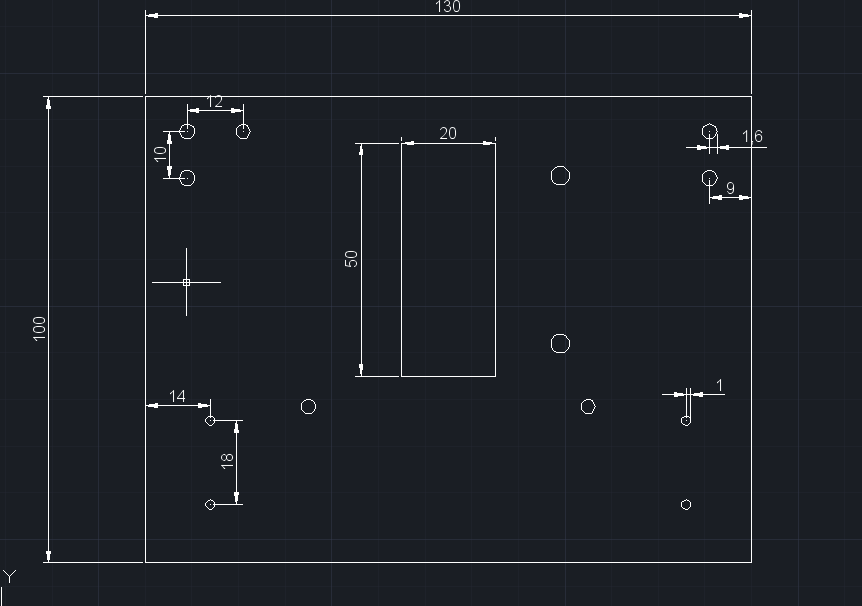
\includegraphics[height=10cm]{figure/procedure/p1}
	\end{center}
 	\caption{CAD drawing \label{fig:cad}}
	\end{figure}
	\item Cut 2 mm-thick carbon fibre board according to the design drawing. Notice: Since only limited information can be illustrated on this figure, you can decide the distance between holes by yourself. You may go through some measurements. There are three types of holes on the board. You can identify them from the size on the figure. The product is as follow. \\
	\begin{figure}
	\begin{center}
	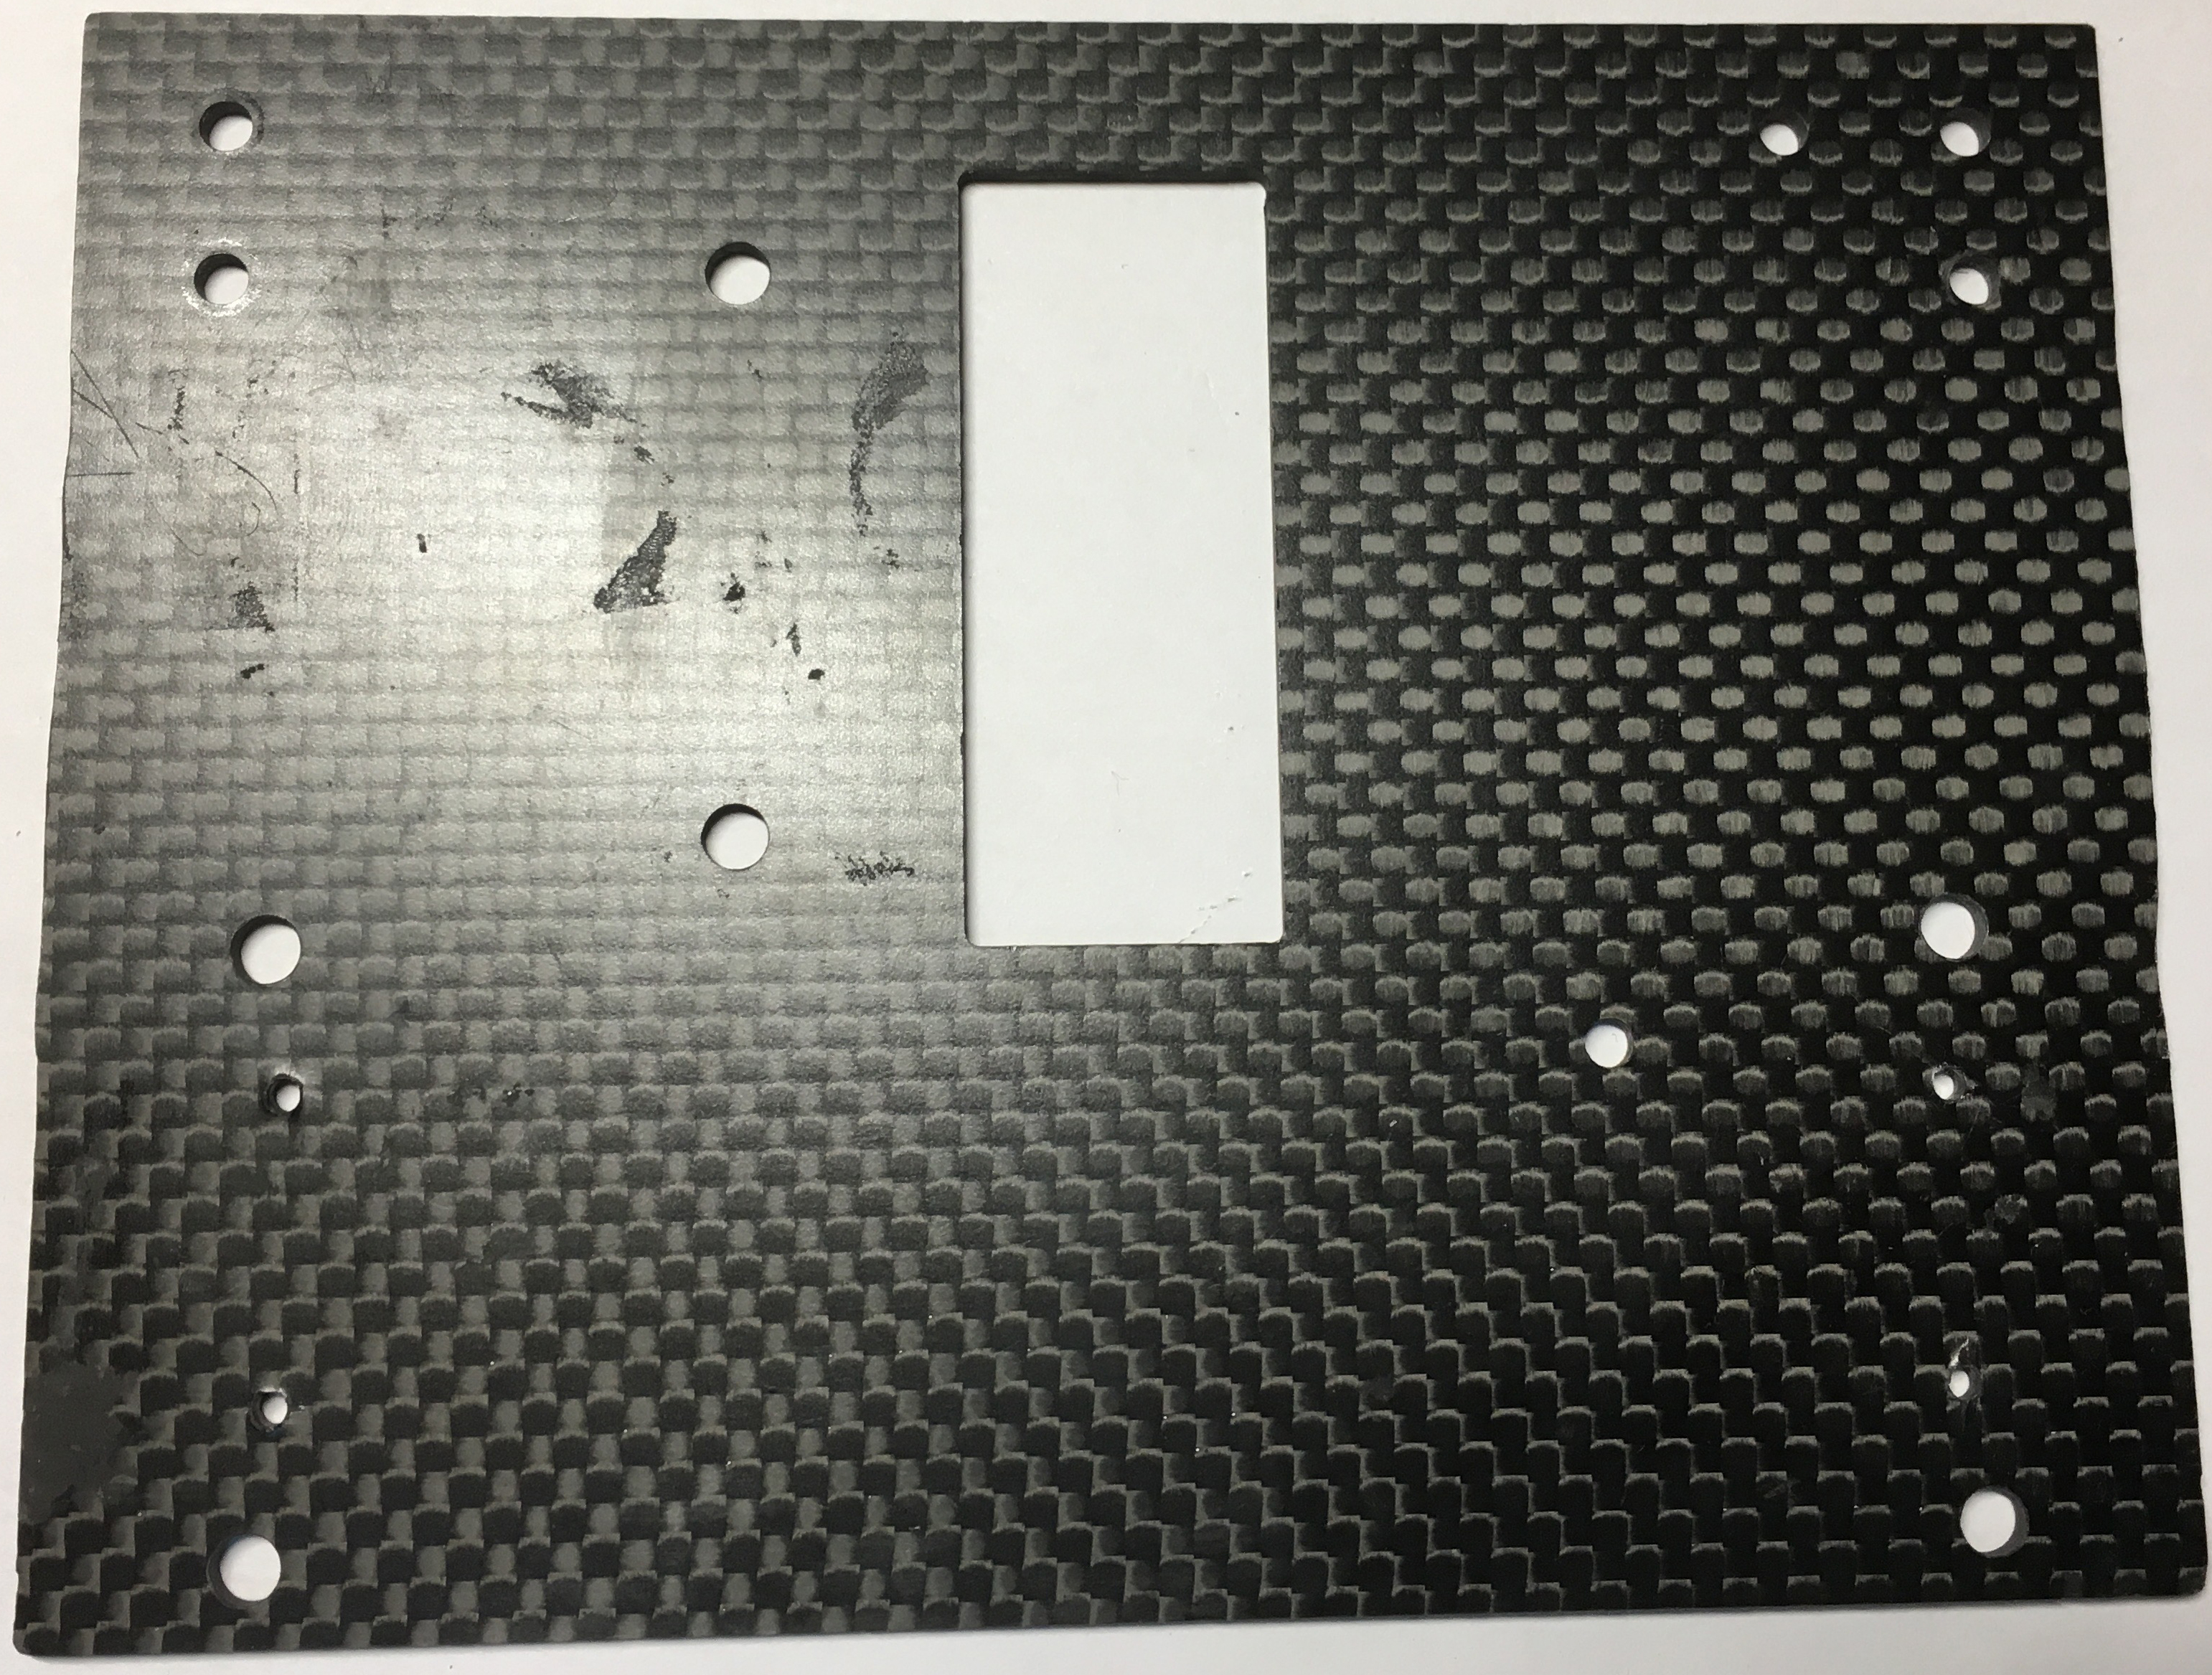
\includegraphics[height=10cm]{figure/procedure/p2}
	\end{center}
 	\caption{Carbon fibre board \label{fig:carbonFiberBoard}}
	\end{figure}
	\end{enumerate}
\item Design circuit diagram 
\item Design wheels
	\begin{enumerate}
	\item Draw a wheel with radius of 2.3 cm on the computer software Solidworks.\\
	\begin{figure}
	\begin{center}
	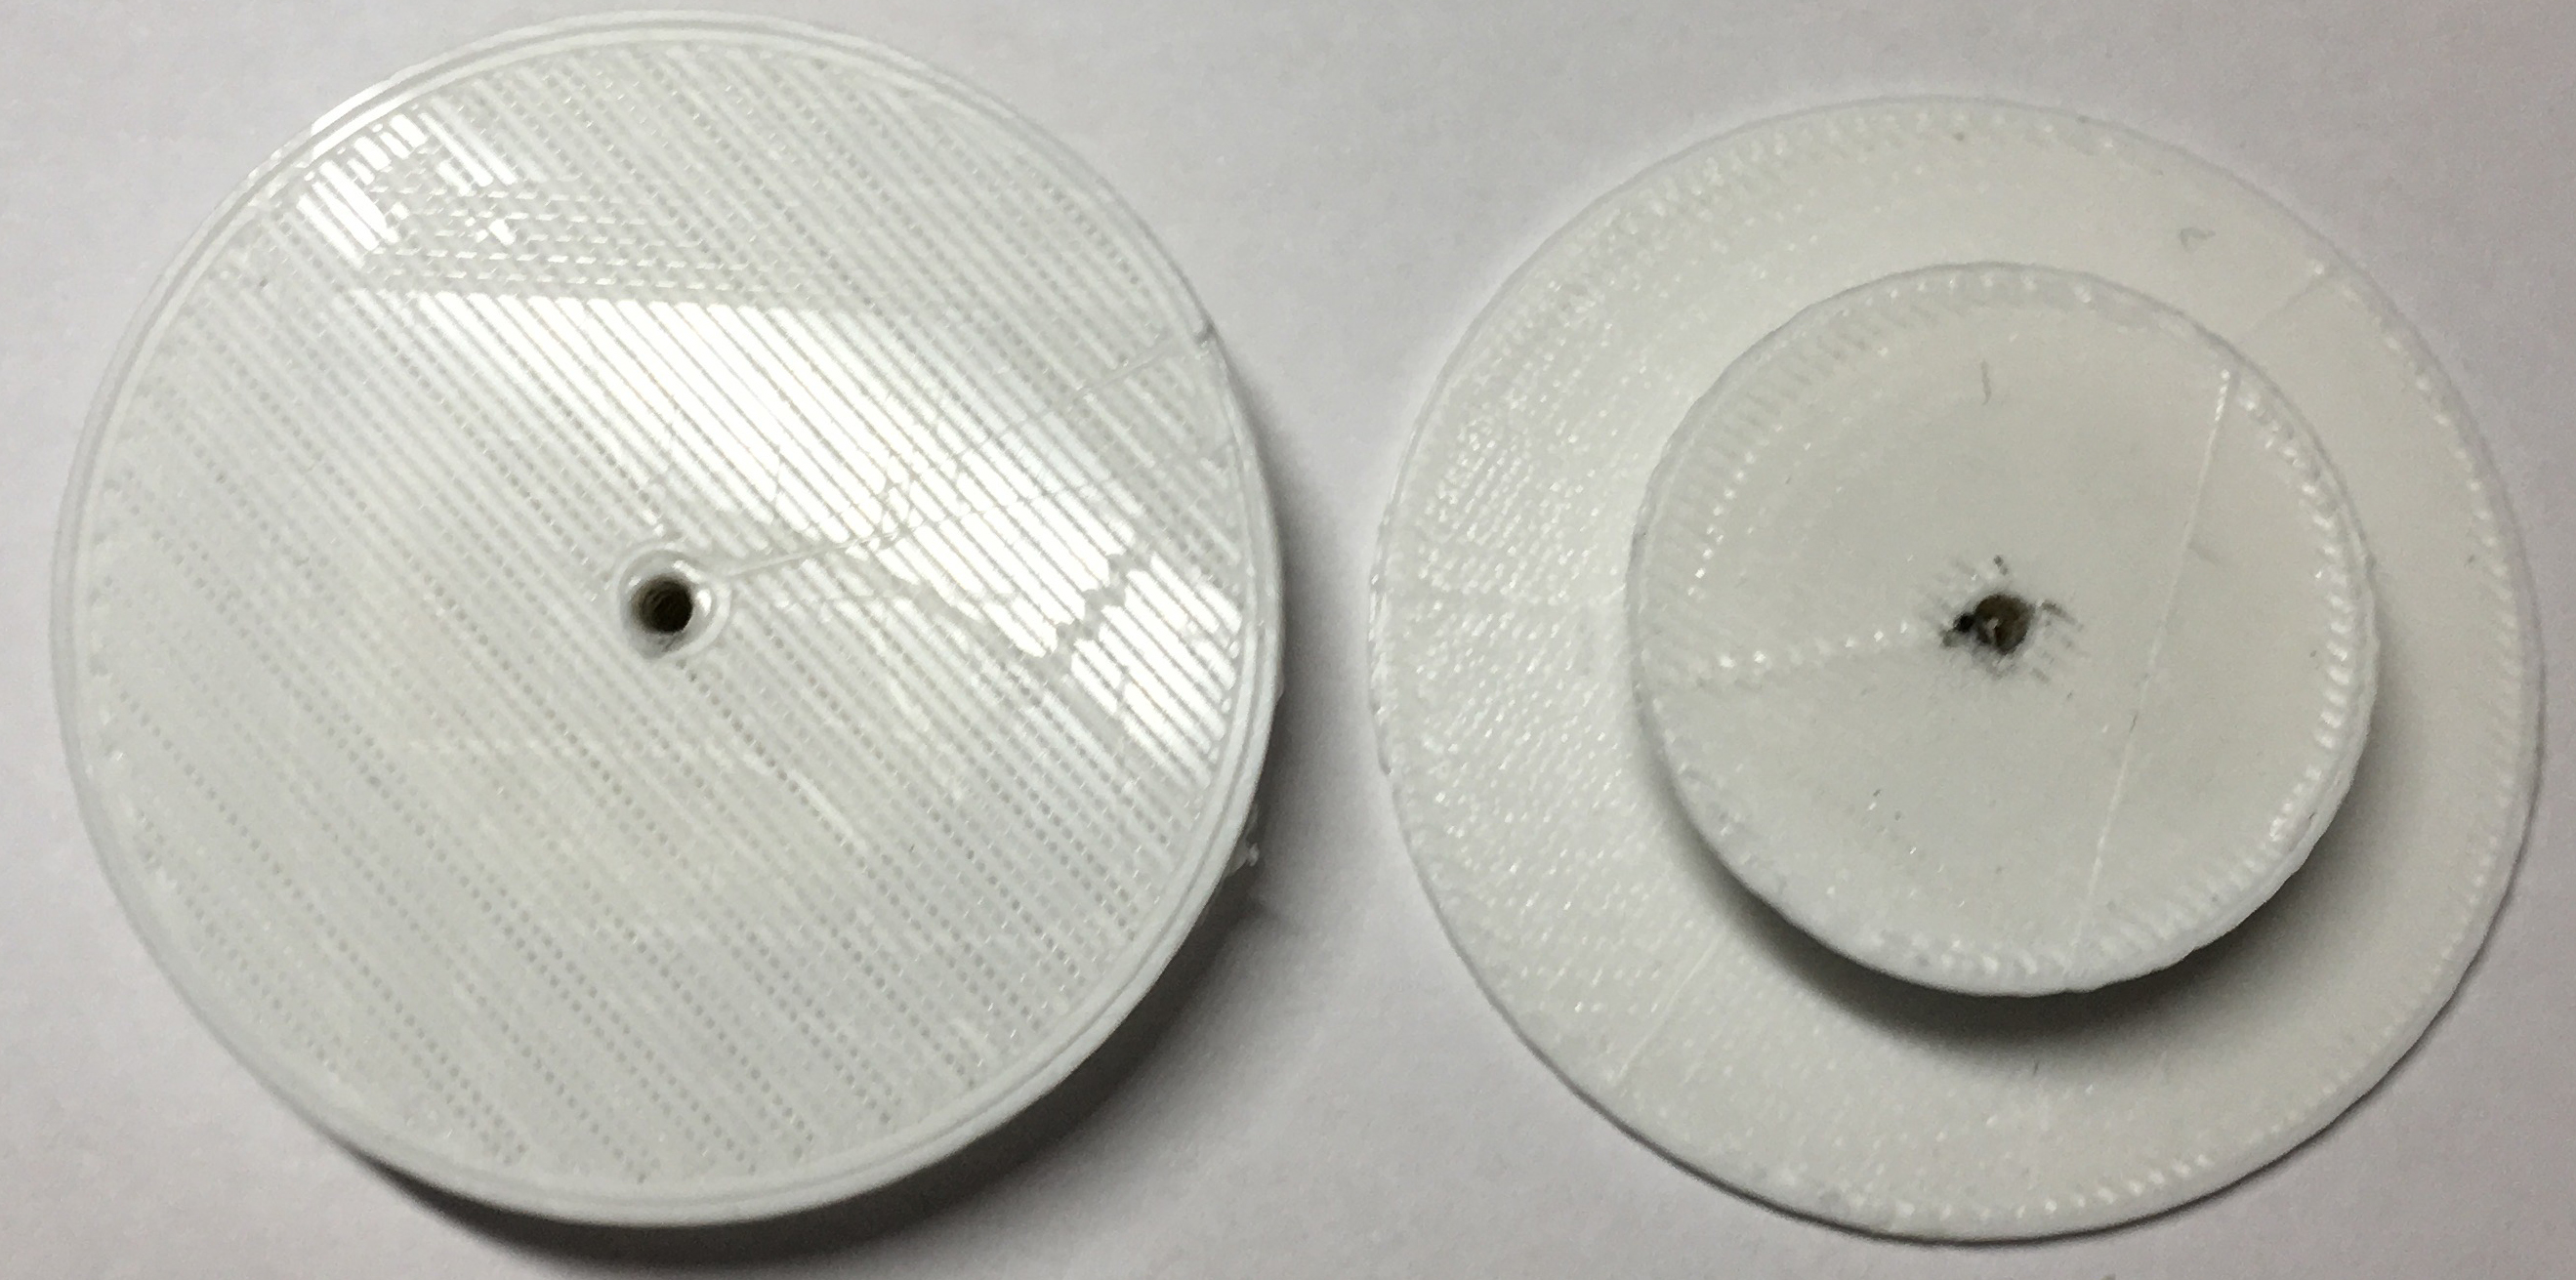
\includegraphics[height=10cm]{figure/procedure/p3}
	\end{center}
 	\caption{Wheels \label{fig:wheels}}
	\end{figure}
	\item Print two wheels according the ``STL'' file in 3D.
	\end{enumerate}
\item Assembling Motor, Servo and Wheels
	\begin{enumerate}
	\item Fix two stators at two corners of the base from below with screws and nuts. 
	\item Fix two N20 motors and back wheels at the other two corners of the base from above with screws and nuts.
	\item Insert a carbon fibre axle in to the hole of the two stators. \textbf{Caution:} Make sure the length on two sides beyond the stators the same. \\
	\begin{figure}[H]
	\begin{center}
	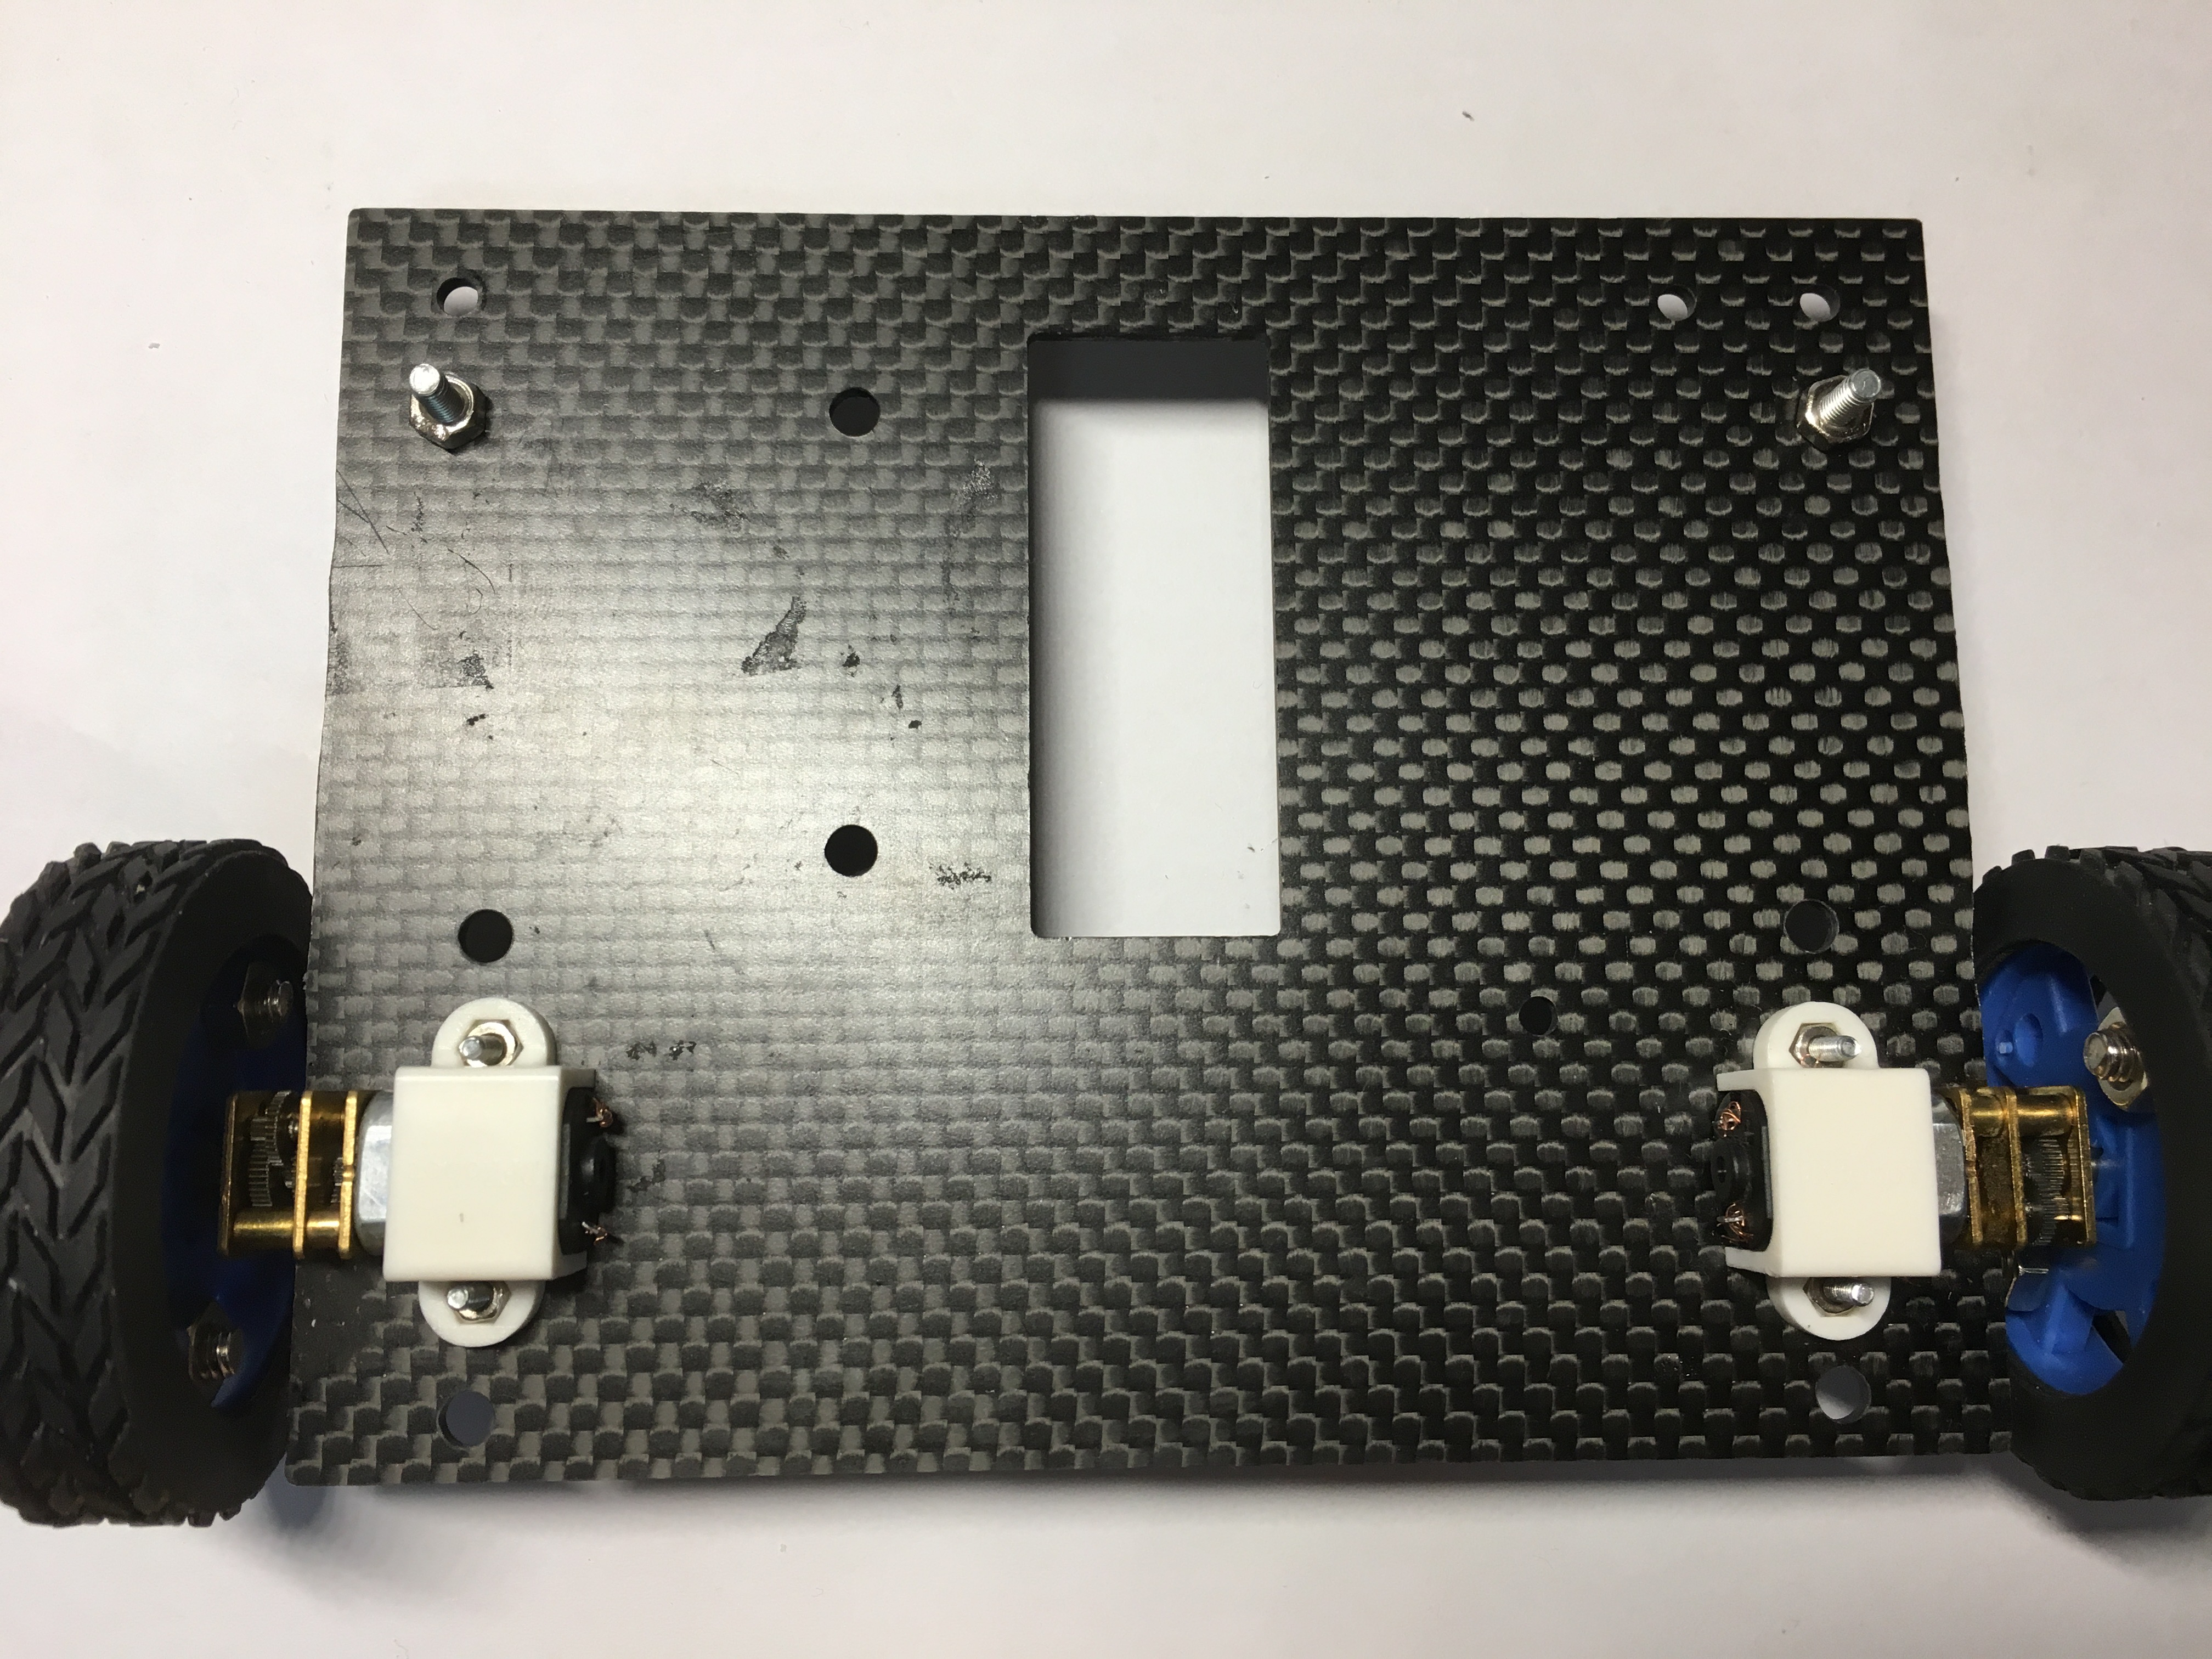
\includegraphics[height=10cm]{figure/procedure/p4}
	\end{center}
 	\caption{Step 4.3 \label{fig:step43}}
	\end{figure}
	\begin{figure}[H]
	\begin{center}
	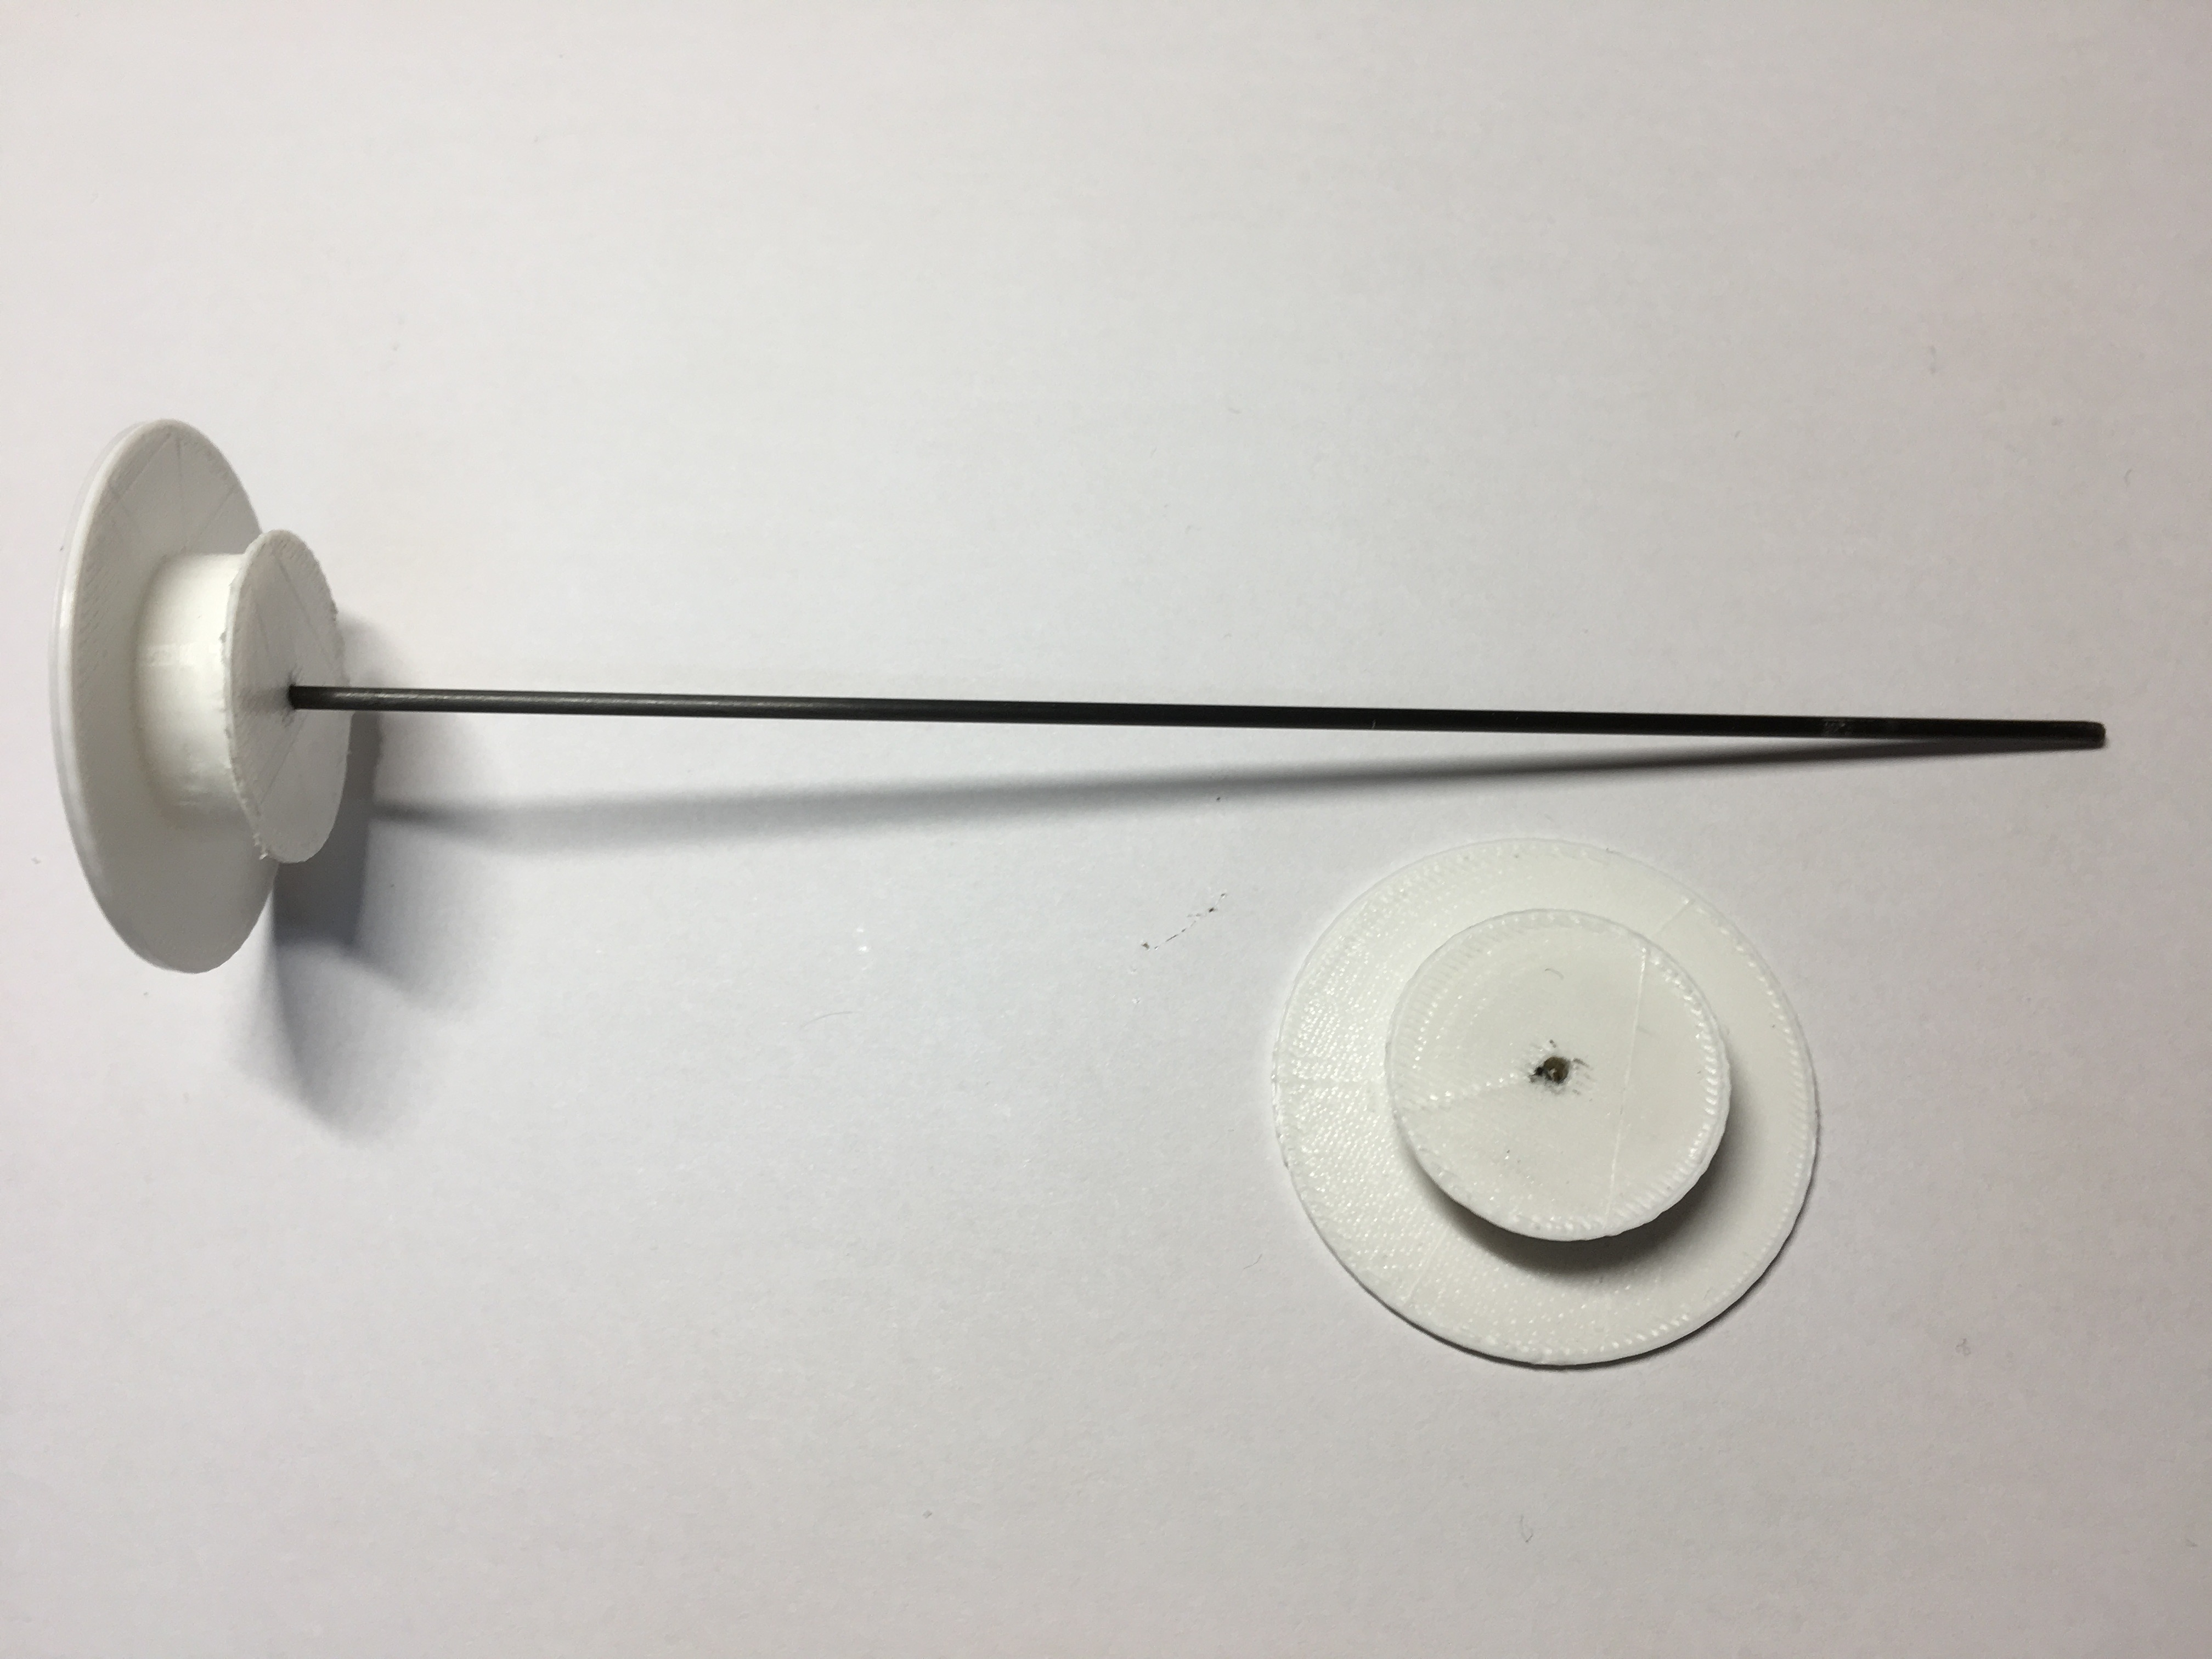
\includegraphics[height=10cm]{figure/procedure/p5}
	\end{center}
 	\caption{Two wheels on the axle. \label{fig:twoWheels}}
	\end{figure}
	\item Insert two wheels onto the axle.
	\item Stick a servo at the base using 3M tape with a steering wheel fixed on it.
	\item Stick a voltage transformer at the back of the base using 3M tape. Caution: Use multiple layers of tape to make sure the transformer strongly sticked to the board.
	\item Stick a battery on the base using 3M tape. \\
	\begin{figure}[H]
	\begin{center}
	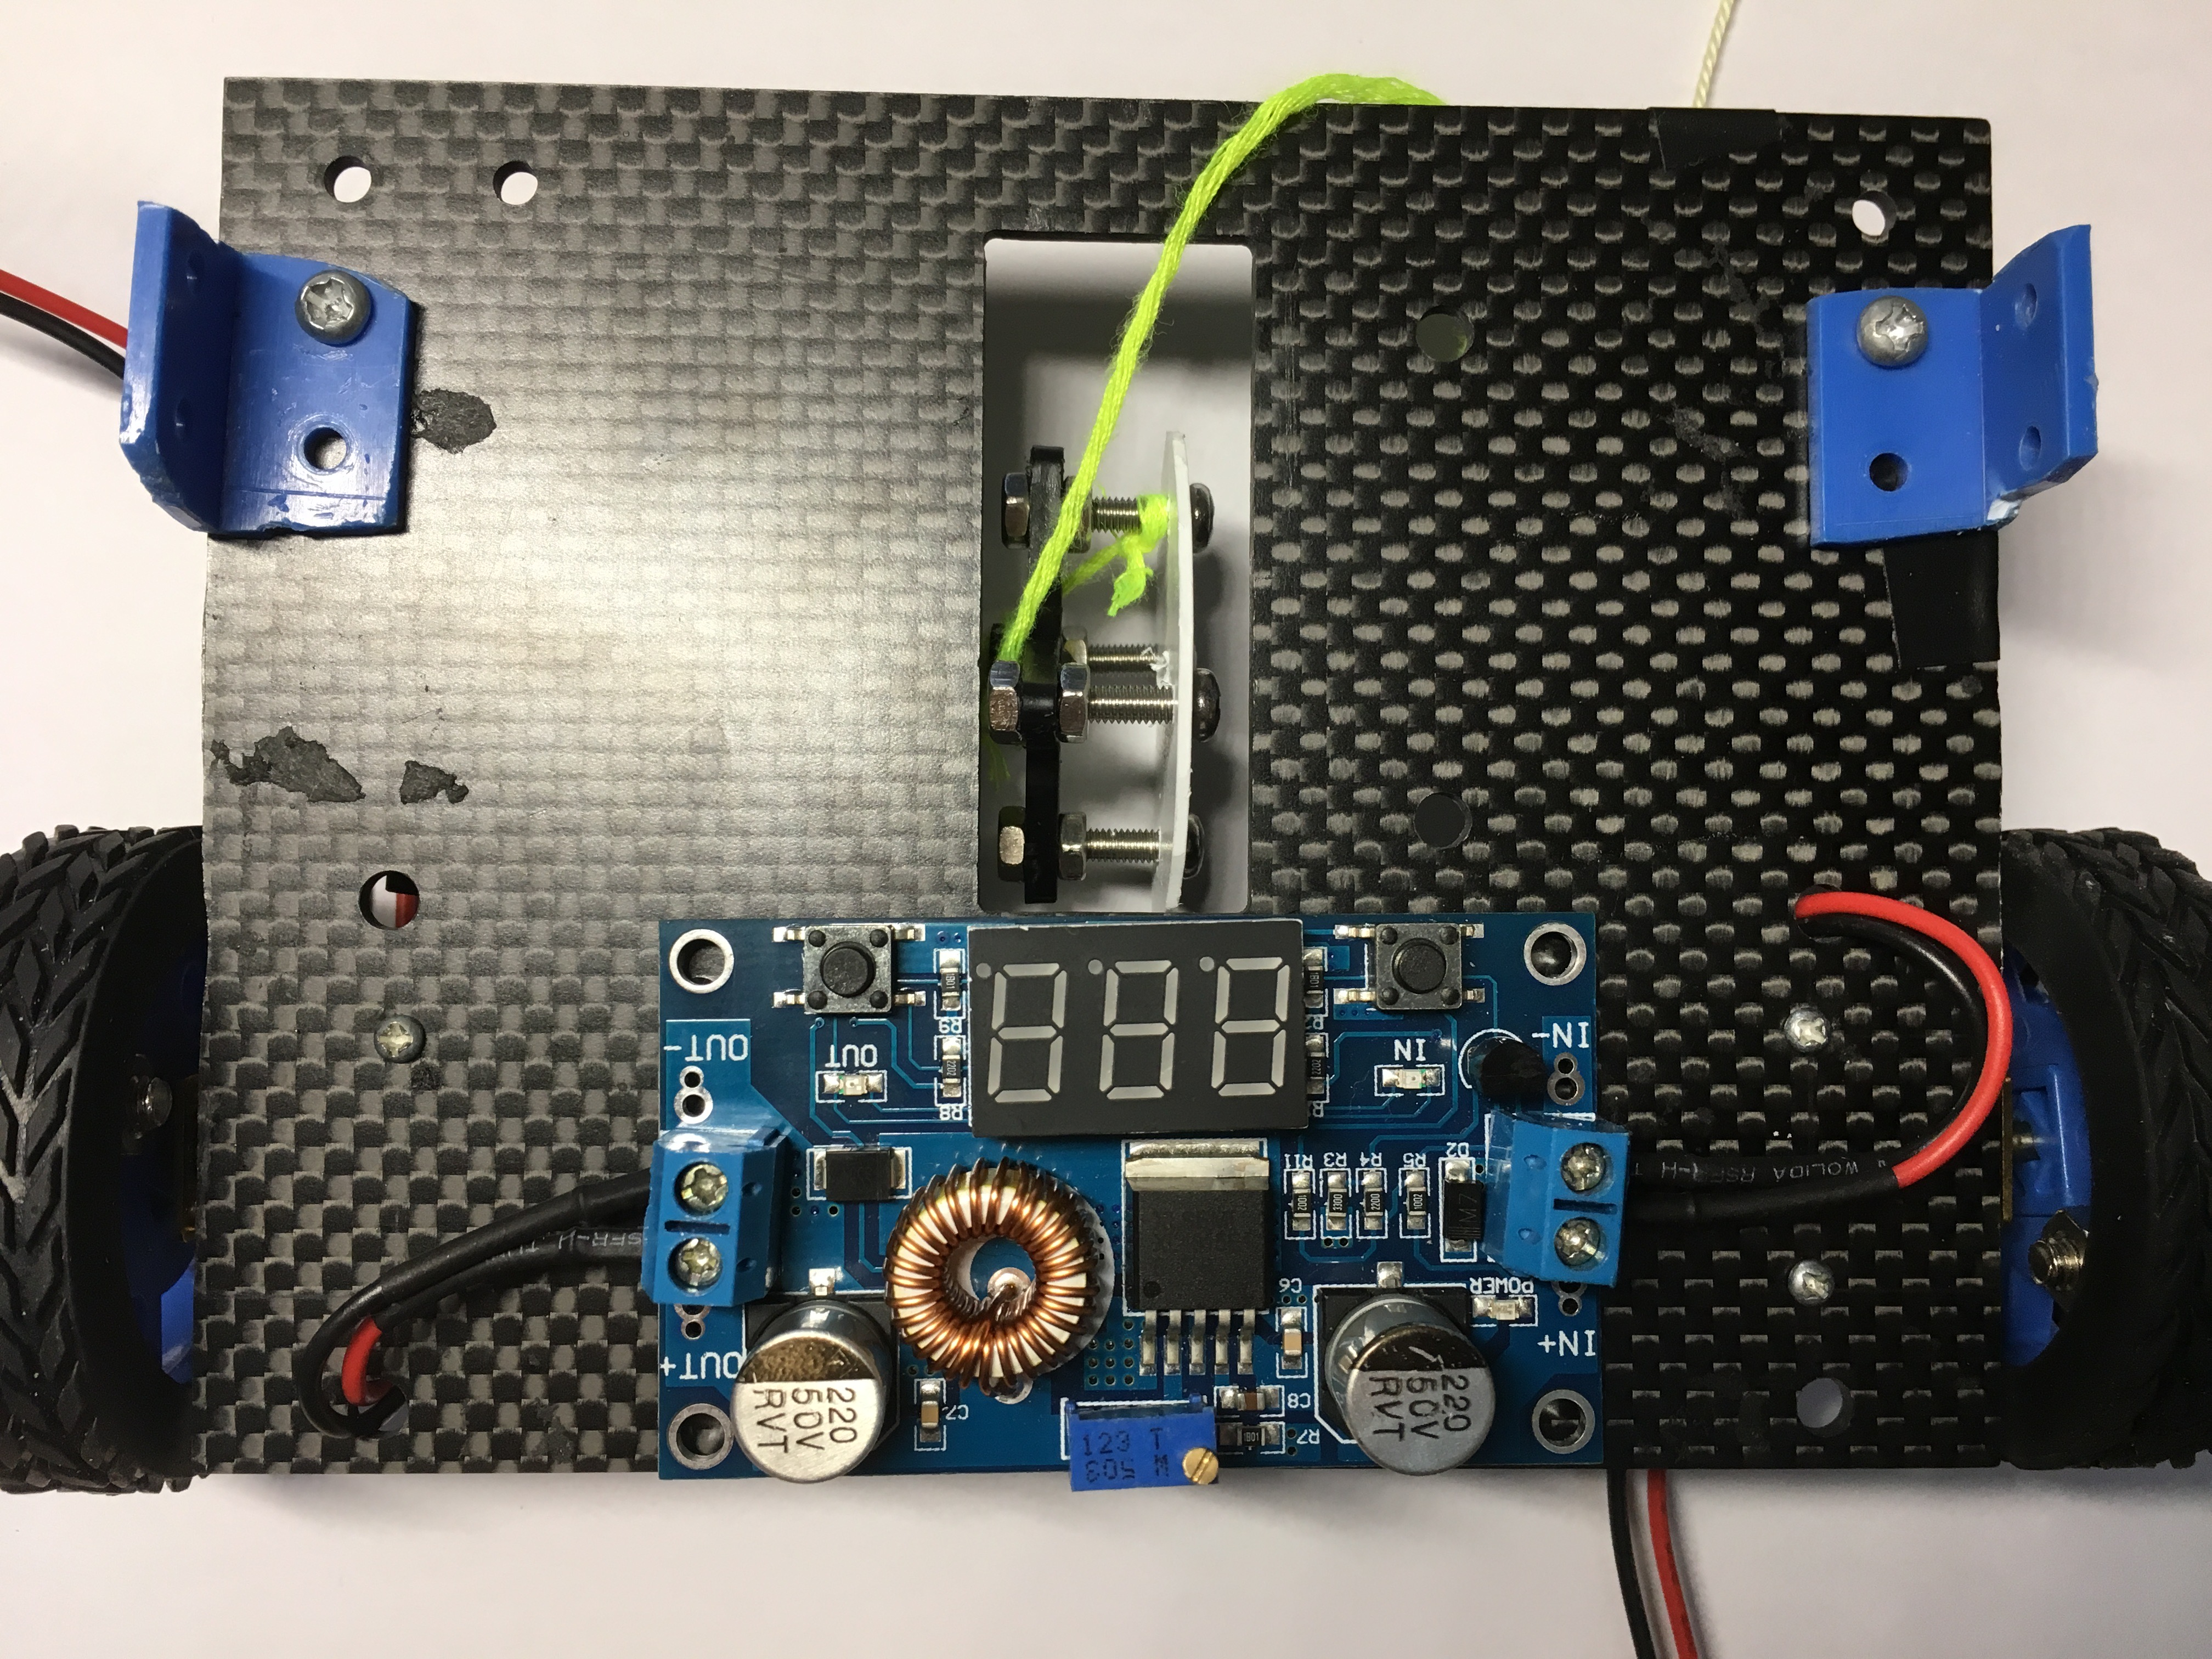
\includegraphics[height=10cm]{figure/procedure/p6}
	\end{center}
 	\caption{Assembling the motor driver. \label{fig:assMotor}}
	\end{figure}
	\item Assembling the motor driver with two motor using tin solder. Caution: tin solder is very dangerous. Do not let your skin contact with tin when it is still hot.\\
	\begin{figure}[H]
	\begin{center}
	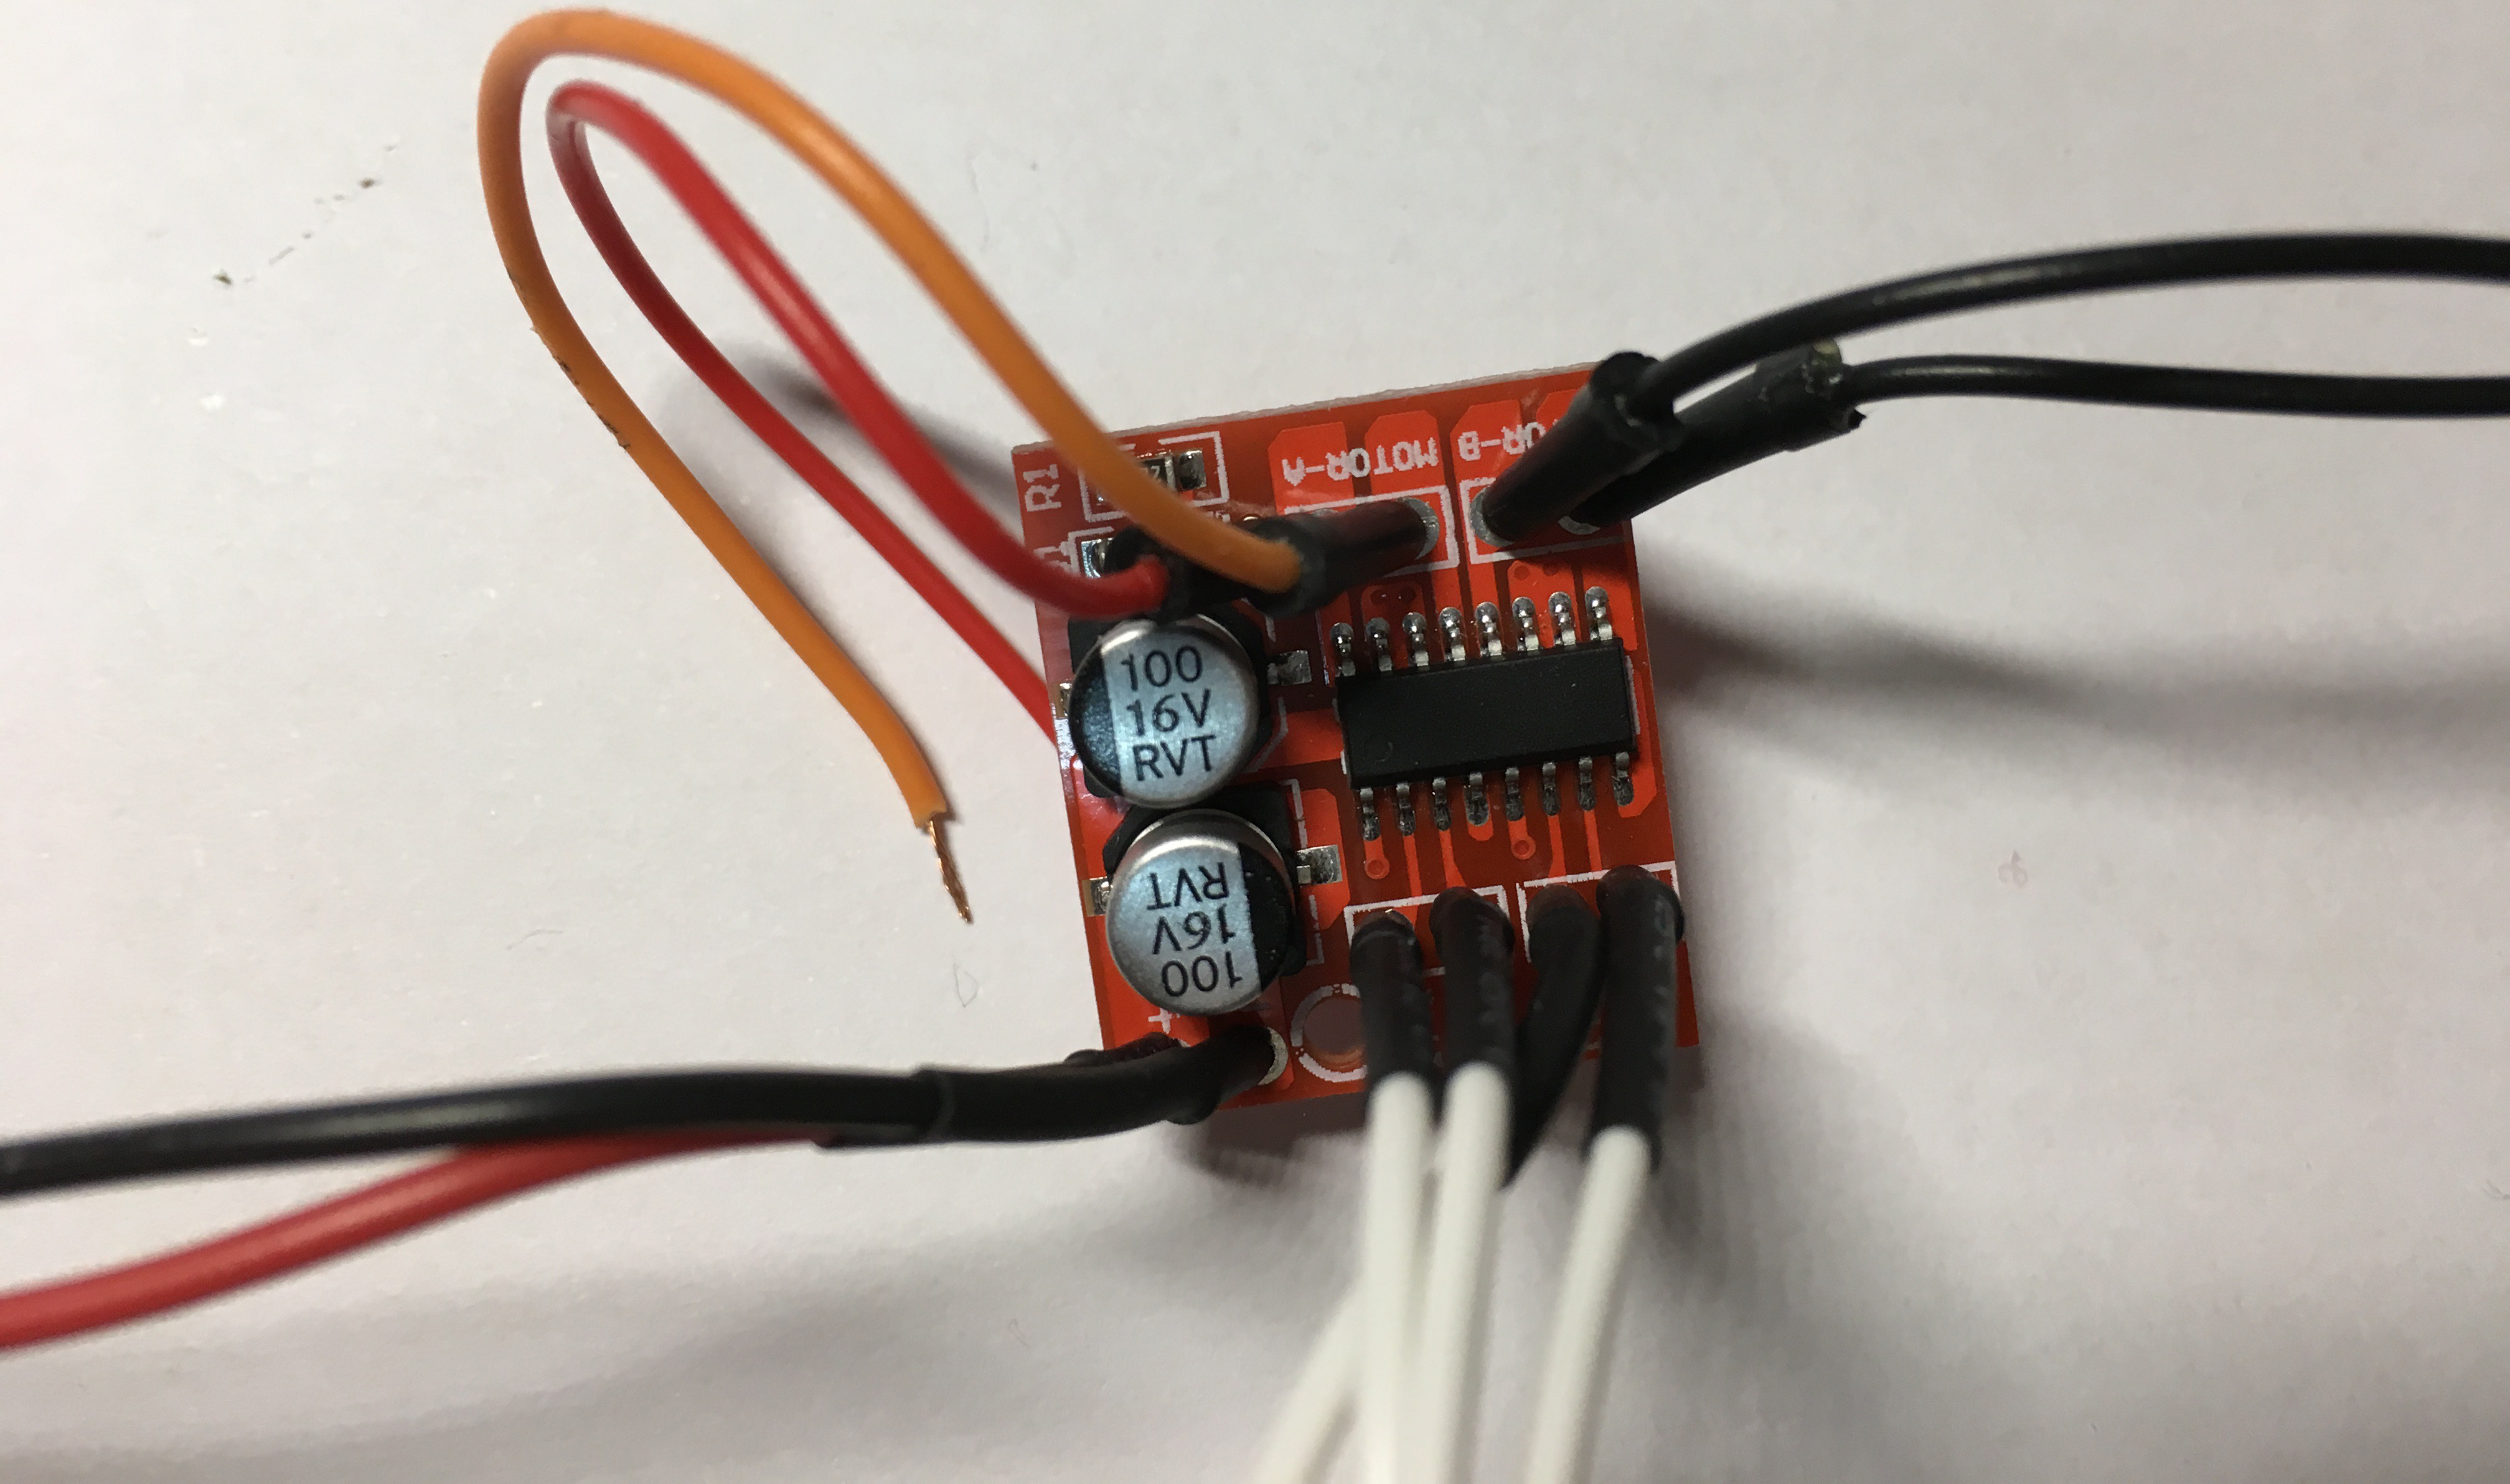
\includegraphics[height=10cm]{figure/procedure/p7}
	\end{center}
 	\caption{Arduino UNO board. \label{fig:ardUnoBoard}}
	\end{figure}
	\item Stick the Arduino UNO board on to the battery using 3M tape.
	\item Finish the assembling according to the circuit diagram. 
	\item Put wires in order and bind them together using Electrical tape. 
	\end{enumerate}
\item Design the rope
	\begin{enumerate}
	\item Make a knot that can adjust the length of the rope.
	\item Bind the rope to the hook. 
	\item Fix them with 502 glue.
	\end{enumerate}
\end{enumerate}
 % procedure
\newpage
\section{Experience Sharing}

\subsection{Bridge}
In the beginning, our group produce paper beams with square cross section to make the first and the second bridge. However, it turns out that this structure is not stable enough to bear the weight of our cart. Then we change our paper from 70 grams per square meter to 80 grams per square meter. According to Professor Shen, a paper beam with rectangular cross section behaves better in carrying a heavy thing, so we decide to give up the previous design and buy new moulds. We complete making our third and fourth bridges before the Game Day. Thanks to the advanced structure, it behaves well on the final stage and surpasses all the other groups.
\par
During the process in making paper bridge, we improve our abilities to use fundamental structure to solve realistic problems and to optimize solutions. Another valuable experience we gain from project one is cooperation and teamwork, especially in producing the paper bridge. We separate the time-consuming task into several parts and assign them to each member. In this way, we manage to produce one bridge after another in high efficiency.
\par
The weight is a problem of our final bridge. It weighs 39.7g. Although the weight still receives full score, a much lighter one can have the same function. We are not able to make more bridges due to the limited time. But for future improvement, we will remake paper beams with two-layer structure and cut down the length of paper pillars.

\newpage

\subsection{Carts}
For the carts part, we mainly focus on the choice of motors and servo. At first, we want to use advanced 130 motor to drive the cart in order to make the speed fast. But the power needed is too much and our motor driver can not afford. So we change to the 180 motor. However, it is heavier and even less powerful. So finally, we choose the N20 DC motor. Though we sacrifice the speed, the torsion becomes bigger. In addition, when we apply the wheels with bigger radius, the speed actually does not decrease. So the N20 motor is more suitable in driving the cart.
\par
In terms of the servo, it is used to lift up the cup. We choose servo instead of motor because assembling servo is much easier than motor. We need another motor driver if the motor is used to lift the cup. But for servo, we don’t have this problem. Also, the torsion the servo can give is also much bigger. Considering the steering wheel has a large radius
$$M=F\times r$$
So when the radius becomes bigger, say ten times. $\frac{dr}{dt}$, which is proportional to the radius would also become ten times. 
\par
Actually, the speed of motor would be greatly influenced due to the torsion. However, when it come to the servo, it works quite well.
 % improvement
\newpage
\section{Appendix} % appendix reference

% =============================

\end{document}